\chapter{Source code}
\label{app:code}

\section{Code Repository}
\label{app:code_repo}

\url{https://github.com/andreasmalling/flixtube}

\section{Docker Images}
\begin{table}[ht]
\centering
    \begin{tabular}{ll}
        \toprule 
        Container           & URL                                                       \\
        \midrule
        \texttt{client}     & \url{https://hub.docker.com/r/andreasmalling/ft_user}     \\
        \texttt{bootstrap}  & \url{https://hub.docker.com/r/andreasmalling/ft_bootstrap}\\
        \texttt{metric}     & \url{https://hub.docker.com/r/andreasmalling/ft_metric}   \\
        \texttt{host}       & \url{https://hub.docker.com/r/andreasmalling/ft_host}     \\
        \texttt{network}    & \url{https://hub.docker.com/r/andreasmalling/ft_network}  \\
        \texttt{plot}       & \url{https://hub.docker.com/r/andreasmalling/ft_plot}     \\
        \bottomrule
    \end{tabular}
\end{table}

\section{Getting Started}
\label{app:getting_started}

\begin{enumerate}
    \item Install \href{https://docs.docker.com/install/}{Docker}, \href{https://docs.docker.com/compose/install/}{Docker Compose}, \href{https://github.com/alexei-led/pumba/releases}{Pumba} and \href{https://www.python.org/downloads/}{Python 3.5}
    \item \href{https://github.com/andreasmalling/flixtube/archive/master.zip}{Download} and unzip the project from the GitHub repository
    \item Navigate into root folder of project
    \item Run \lstinline[columns=fixed]{./run.py envs/exp.env} for a simple experiment or check out \lstinline[columns=fixed]{./run.py --help} for more options
    \item ????
    \item PROFIT!!!
\end{enumerate}
\newpage
\section{Video Demonstration}
Video of demo run with a default stable network and an experimental introduction of 10 Bingers over 60 seconds. This experiment corresponds to \expid{B10}.

\begin{figure}[htbp]
    \myfloatalign
    \href{https://www.youtube.com/v/_88_Kb7C6FY?rel=0}{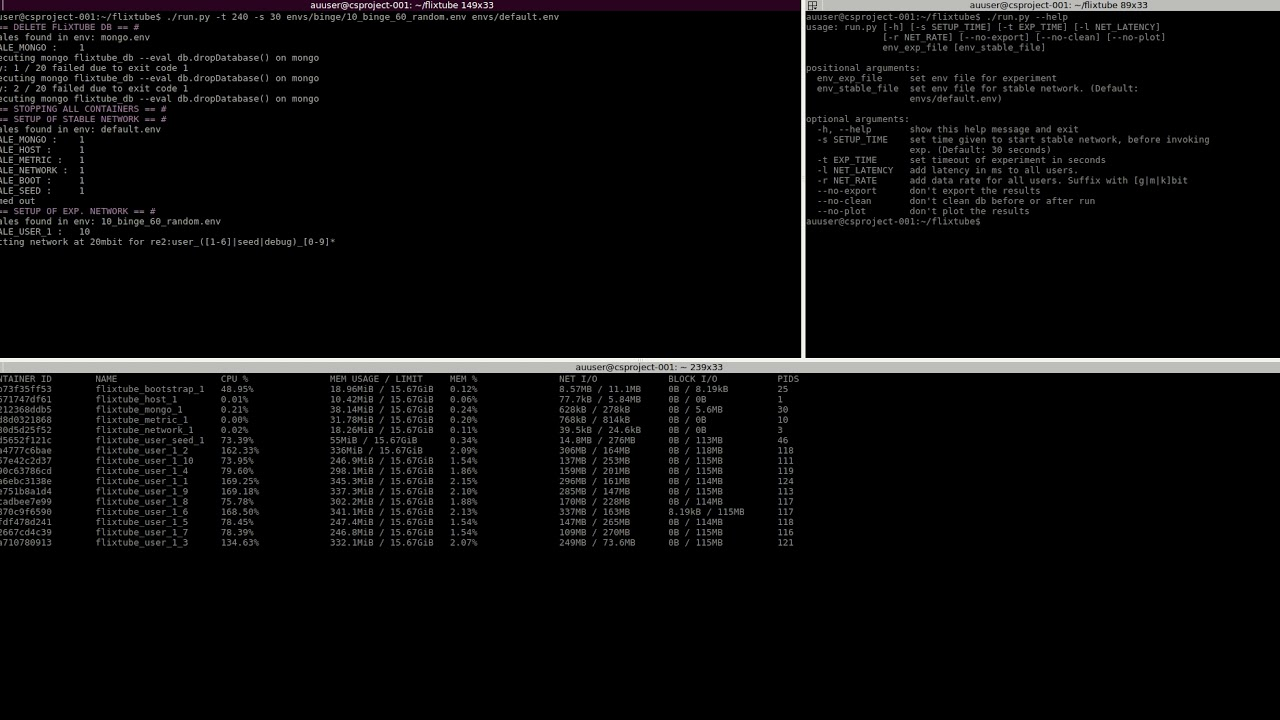
\includegraphics[width=\linewidth]{gfx/demo.jpg}}
    \caption*{Video can be found at \url{https://youtu.be/_88_Kb7C6FY}}
    \label{vid:demo_b10}
\end{figure}
